\documentclass[preprint, aps]{revtex4-1}

%------------------------------------------------------------------------------%
%--------------------------------  Preamble  ----------------------------------%
%------------------------------------------------------------------------------%

\usepackage{amsmath}    % need for subequations
\usepackage{graphicx}   % need for figures
\usepackage{color}      % use if color is used in text
\usepackage{subfig} 	% use for side-by-side figures
\usepackage{float}		% keep floats in place
\raggedbottom           % don't add extra vertical space

\graphicspath{ {figures/} }

%------------------------------------------------------------------------------%
%--------------------------------  Document  ----------------------------------%
%------------------------------------------------------------------------------%

\begin{document}

%------------------------------------------------------------------------------%
%-------------------------------  Title page  ---------------------------------%
%------------------------------------------------------------------------------%

\title{Computational studies of defect mediated transport}
\author{Bryan Chem}
\affiliation{University of Minnesota Twin Cities, School of Physics and 
	Astronomy, Minneapolis, MN 55455}
\date{\today}

\begin{abstract}
Using a molecular dynamics simulation, a system in which a sphere is submerged 
in a liquid crystal consisting of 4096 molecules is simulated. The ellipsoidal 
molecules tend to anchor perpendicularly to the surface of the sphere. This
anchoring induces a defect and causes long range distortions in the 
otherwise aligned liquid crystal molecules. Upon equilibration of the system, 
the configuration of the sphere and the associated defect are examined. The 
distance the defect forms from the surface of the sphere is specifically of 
interest. The geometry of configuration dictates the dynamical behavior of the 
sphere in the liquid crystal.

\end{abstract}

\maketitle

\tableofcontents

\newpage
%------------------------------------------------------------------------------%
%------------------------------------------------------------------------------%
%------------------------------------------------------------------------------%

\section*{Introduction}
Due to being a uniaxial fluid, liquid crystals have a wide variety of 
behavior distinct from that of an isotropic fluid whose molecules do not have
ordering. Formation of defects and the resulting effects on the transport 
properties of liquid crystals allow for precise control of the flow of particles
suspended in the liquid crystal itself. In this study, the equilibrium
configuration of a system where a sphere is immersed in a liquid crystal is
examined in order to gain insight on the behavior of the system in the dynamic
situation. Systems where particles are suspended in a liquid crystal are called
nematic suspensions. 

Due to the anisotropic (directionally dependent) properties of liquid crystals, 
the immersed particles exhibit particularly interesting transport properties 
under an applied electric field that would not otherwise be seen in an isotropic 
fluid. Liquid crystal molecules, which are ellipsoidal in shape, tend to anchor 
perpendicularly to the particles. Due to imposed boundary conditions, defects 
form inside of the liquid crystal itself. These induced defects in the liquid 
crystal medium govern the behavior of suspended particles by distorting the 
orientations of the molecules and, as a result, increasing its resistance to
flow. In theory, there are two types of defects may form after a sphere has been 
immersed in the liquid crystal. These are shown in Figure 
\ref{fig:defect-config}. The first is a line defect that circles the sphere, 
and the second is a point defect that forms close to the sphere. In experiment, 
the dipole configuration with two point defects is observed \cite{lubensky98}. 
For systems where sphere is small relative to the length of the molecules, the
line defect is observed. For large spheres, the point defect is observed.
	\begin{figure}[H]
		\centering
		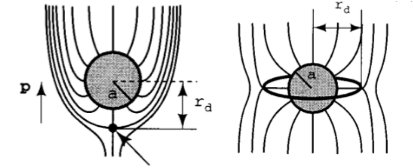
\includegraphics[width=0.7\textwidth]{defect-config.png}
		\caption{Two expected defect configurations as seen in 
		\cite{lubensky98}}
		\label{fig:defect-config}
	\end{figure}

The equilibrium configuration of the sphere and defect are simulated using a
technique called molecular dynamics. The distance between the immersed sphere 
and the corresponding defect in the equilibrium configuration will give 
information about the ability of the sphere to flow in the liquid crystal. 
Larger, more abrupt changes in the orientations of the molecules will increase 
the resistance of the system to flow \cite{billeter00}. Thus, a smaller distance
indicates that there will be more resistance to flow than if the sphere and
defect were further away from each other.

These systems are especially of interest because of their applications in flow 
control. Immersed particles can be translated inside of the liquid crystal
molecules by applying an electric field \cite{conklin17}. 

\subsection*{Liquid crystals}
A liquid crystal is an intermediate state of matter that possesses properties of 
both liquids and crystals. It can flow and form droplets like a liquid, but it 
also has anisotropic, directionally dependent, properties. This means that 
unlike an isotropic fluid, where the viscosity is constant, the viscosity of a 
liquid crystal will change depending on the orientation of the molecules 
relative to the flow. A popular application of liquid crystals is in liquid 
crystal displays that exploit their anisotropic electrical and optical 
properties. These properties are the result of different levels of ordering in 
the orientation and position of the constituent molecules.

Molecules that make up a liquid crystal tend to have a well defined long axis 
and short axis. In practice, these molecules are modeled as ellipsoids. These 
ellipsoids are axially symmetric which will have ramifications later on when 
choosing an appropriate order parameter to characterize the liquid crystal. 

Typical phases of liquid crystals include the isotropic, nematic, and smectic 
phases. In an isotropic phase, there exists no order in the orientation or 
position and for all intents and purposes is an isotropic fluid. The nematic 
phase is characterized by the molecules having orientational order and aligning 
along a vector called the director. This is the phase of interest in this study. 
At lower temperatures, the smectic phase forms which displays both orientational
order and also order in the positions of the center of masses of the particles
\cite{andrienko06}.
	\begin{figure}[H] 
		\centering
		\subfloat[]{
			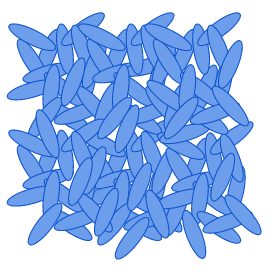
\includegraphics[width=0.3\textwidth]{isotropic.png}
		}
		\subfloat[]{
			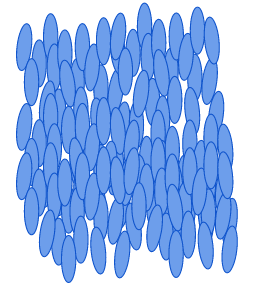
\includegraphics[width=0.3\textwidth]{nematic.png}
		}
		\subfloat[]{
			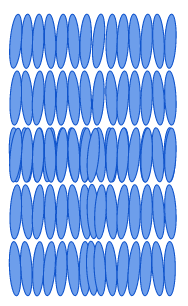
\includegraphics[width=0.2\textwidth]{smectic.png}
		}
		\caption{(a) Isotropic phase: No orientational or positional ordering
		-for all intents and purposes behaves like an isotropic fluid (b)
		Nematic phase: Orientational ordering but no positional ordering (c) 
		Smectic phase: Orientational and positional ordering}
		\label{fig:phases}
	\end{figure}

In the nematic phase, the ideal or most energetically favorable configuration is
 one where all of the molecules are perfectly aligned with each other (although 
not positionally correlated). In practice, this configuration is 
never realized and there exists small fluctuations in the orientation of the 
molecules \cite{degennes95}.

\subsection*{Topological defects}
Additionally, defects in liquid crystals allow for the control of particles 
transport in the liquid crystal itself. Within ordered materials (materials 
where we can assign an order parameter at each point in space), there is always 
the possibility of defects forming. Defects form during phase transitions,
through the introduction of colloidal molecules, and external forces among other 
things. Defects are areas inside materials where the configurations of the 
molecules change drastically. Furthermore these defects, cannot be removed from 
the material by a simple transformation \cite{mermin79}. Examples of defects in 
liquid crystals are seen in Figure \ref{fig:defects}.
	\begin{figure}[H]
		\centering
		\subfloat[]{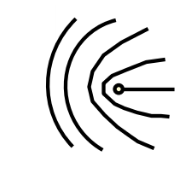
\includegraphics[width=0.3\textwidth]{plus-line.png}}
		\subfloat[]{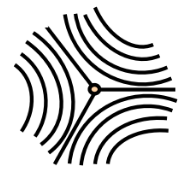
\includegraphics[width=0.3\textwidth]{minus-line.png}}

		\subfloat[]{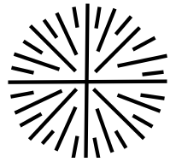
\includegraphics[width=0.3\textwidth]{plus-point.png}}
		\subfloat[]{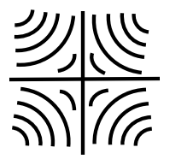
\includegraphics[width=0.3\textwidth]{minus-point.png}}
		\caption{(a) A $+\frac{1}{2}$ line defect (b) A $-\frac{1}{2}$ line
		defect (c) A $+1$ point defect (d) A $-1$ point defect. Figures from
		\cite{chuang91}}
		\label{fig:defects}
	\end{figure}

In order to classify defects, the sum of the change in angle about a closed 
circuit surrounding the defect is taken as shown in Figure \ref{fig:circuit}. 
The result of the sum after being divided by a factor of 2$\pi$ is called the 
topological charge or winding number.
	\begin{equation} \label{topological-charge}
		2\pi s = \oint d\theta
	\end{equation}
In liquid crystals, the two types of observed defects are line defects and point
defects. Line defects have topological charge of $\pm\frac{1}{2}$, and point 
defects have topological charge of $\pm1$ \cite{lubensky98}. 
	\begin{figure}[H]
		\centering
		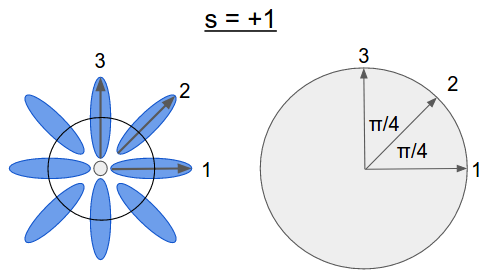
\includegraphics[width=0.6\textwidth]{circuit-calc.png}
		\caption{Calculation of the topological charge of a radial hedgehog
		defect}
		\label{fig:circuit}
	\end{figure}
Interestingly enough, taking the integral along any closed contour only 
containing the defect will result in the same topological charge. This implies 
that the defect not only disturbs the director field locally, but has long range
effects on the orientation of molecules far away from it. Since the orientation
of the molecules relative to the flow affects the liquid crystals viscosity 
these defects have a large impact on the transport properties.

\subsection*{Nematic suspensions}
When a sphere is immersed in the liquid crystal, the molecules will anchor 
perpendicular to the sphere. Calculating the integral in 
\ref{topological-charge} by taking the integral along a closed circuit 
surrounding the sphere, it turns out that the sphere has a topological
charge of $+1$, and it mimics a radial point defect.

If the molecules are forced to anchor as shown in Figure \ref{fig:bc}, it is 
possible to force the topological charge of the liquid crystal to be conserved. 
If there was only a $+1$ defect inside of the system the director field would be
discontinuous at the boundary which is not energetically favorable. As such, a
$-1$ defect is induced as it is more energetically favorable \cite{stark01}.
	\begin{figure}[H]
		\centering
		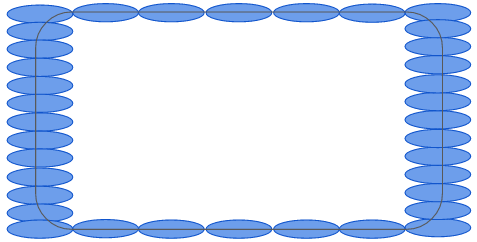
\includegraphics[width=0.5\textwidth]{bc.png}
		\caption{Boundary conditions of the system. There is no change in angle,
		so the topological charge at the boundary is zero}
		\label{fig:bc}
	\end{figure}

\subsection*{Order parameter}
To measure the properties of the liquid crystals in the molecular dynamics 
simulation, an order parameter must be specified. Many properties of liquid
crystals depend on the local average orientations of the molecules. An order
parameter should be able to calculate this. A vectorial order parameter cannot 
be used in the case of liquid crystals due to the axial symmetry of the 
molecules. It is not possible to calculate an average orientation because the 
addition of the orientation of two molecules in the "opposite" direction would 
equal zero. Thus, the local average orientation would cancel to zero
everywhere in the liquid crystal. It is necessary to use a tensor order 
parameter. 

For a small but still macroscopic volume, the Q-tensor is
	\begin{equation} \label{q-tensor}
		Q = \frac{1}{N} \sum_{i}^{N} 
		(e_{\alpha}^{(i)} e_{\beta}^{(i)} - \frac{1}{3}\delta_{\alpha\beta})
		= \frac{1}{N} \sum_{i}^{N}
		\begin{bmatrix}
			e_x^{(i)}e_x^{(i)} - \frac{1}{3} 
			& e_x^{(i)}e_y^{(i)} 
			& e_x^{(i)}e_z^{(i)} \\

			e_y^{(i)}e_x^{(i)} 
			& e_y^{(i)}e_y^{(i)} - \frac{1}{3} 
			& e_y^{(i)}e_z^{(i)} \\

			e_z^{(i)}e_x^{(i)} 
			& e_z^{(i)}e_y^{(i)} 
			& e_z^{(i)}e_z^{(i)} - \frac{1}{3}
		\end{bmatrix}
	\end{equation}
$e^{(i)}$ is the orientation of a molecule in the volume being used to calculate
the tensor. 

The tensor order parameter is symmetric and traceless by construction. The 
result is that the diagonalized tensor has a specific form:
	\begin{equation*} \label{diag-q-tensor}
		Q_{diag} = 
		\begin{bmatrix}
			-\frac{1}{3} S - \eta 
			& 0 
			& 0 \\
			0 
			& -\frac{1}{3} S + \eta 
			& 0 \\
			0 
			& 0 
			& \frac{2}{3} S
		\end{bmatrix}
	\end{equation*}
After diagonalizing the Q-tensor, the eigenvector corresponding to the largest
eigenvalue is the director for the small but macroscopic volume element. These
eigenvectors once calculated for the whole liquid crystal can be used to create
a director field which maps the local preferred orientations throughout the
system. 

$S$ is the scalar order parameter which gives a general measure of alignment 
and $\eta$ is a measure of biaxiality. $S=0$ indicates a completely isotropic 
alignment of the molecules in the volume element. $S=1$ indicates a completely 
uniform alignment of the molecules along a single axis. A non zero $\eta$ is an 
indicator of biaxial alignment in the volume of molecules. A large $\eta$ 
indicates that there may be more than one preferred axis of alignment
\cite{degennes95}.

\subsection*{Biaxial coefficient}
Additionally, using the tensor order parameter, it is possible to find defects 
inside the liquid crystal using a defined coefficient -the biaxial coefficient. 
The biaxial coefficient is
	\begin{equation} \label{biaxial}
		\beta = \frac{(detQ)^2}{(TrQ^2)^3} - \frac{1}{54}
	\end{equation}
When the molecules are uniaxially aligned, the coefficient is zero. For any
regions of space where there may be more than one preferred axis of alignment,
it is non-zero. The calculation above is convenient because the tensor order
parameter does not need to be diagonalized in order to compute the biaxial
coefficient.

\section*{Computational details}

\subsection*{Molecular dynamics}
Molecular dynamics is a method of simulating the behavior of a system of 
particles interacting under a potential by integrating Newton's equations of 
motion. Three items are necessary in order to construct a molecular dynamics 
simulation. To begin the simulation, parameters such as the desired temperature
and density for the system must be specified. A model potential is needed
to describe the interaction of a particle with its neighbors. After finding all
of the forces and torques using the model potential, a numerical method of
integrating the equations of motion for each particle is needed. This 
integration should use a particle's current position and momentum, along with 
the calculated forces and torques acting upon it, to advance the particle to a 
new position at a subsequent time step. 	   

Solely using a pair potential to model the interactions of a system of atoms, it
is actually possible to simulate a liquid. A pair potential describes the 
potential energy in the configuration of two atoms. The Lennard-Jones potential is a common pair potential used in molecular dynamics simulations,
	\begin{equation} \label{lennard-jones}
		V^{LJ}=4\epsilon
		\left[
		\left(\frac{\sigma}{r}\right)^{12}
		- \left(\frac{\sigma}{r}\right)^6
		\right]
	\end{equation}
$\epsilon$ is the well depth parameter which specifies the strength of the
interactions. $\sigma$ is the distance parameter which specifies when the
gradient of the potential becomes positive and the forces become repulsive.
The potential has an attractive tail (modelled by the negative term) that
represents the van der Waals force and a repulsive core (modelled by the
positive term) that represents the repulsion from particles colliding with each 
other. The two terms together form a potential well which allows the particles 
to "stick" to each other and form liquid phases. 

In order to model a system of liquid crystals, an anisotropic pair 
potential that accounts for the relative orientation of the particles is 
necessary.
	
Once the potential is known, the forces on an individual particle $i$ due to a 
particle $j$ can be calculated by taking the negative gradient of the potential 
as shown below.
	\begin{equation} \label{force}
		\mathbf{f}_{ij}=-\nabla_{r_{ij}}V_{ij}
	\end{equation}
The torque, given an anisotropic potential, on a particle $i$ due to a particle 
$j$ is given by,
	\begin{equation} \label{torque}
		\mathbf{\tau}_{ij}=-\mathbf{e_i}\times\nabla_{\mathbf{e}_{i}}V_{ij}
	\end{equation}
$\mathbf{e}_{i}$ is the orientation of particle $i$. Thus, the total force and 
total torque on a particle is the sum of all of forces and torques exerted by 
the other particles in the system. In practice, a cuttoff distance is specified 
in order to make the calculations less cumbersome computationally.
	
When choosing a method to numerically integrate Newton's equations of motion, 
some considerations to be taken are choosing a method that is time-reversible 
and conserves the energy, the accuracy of the method, and the largest allowable 
time step. The time reversibility and conservation of energy criteria are 
necessary to ensure that the system behaves in a realistic manner. The accuracy 
of the algorithm is less important. There will undoubtedly be small error in the 
integration, but these errors have not been proven to effect the validity of the 
results obtained from molecular dynamics simulations. Finally a large time step
allows for more efficiency by allowing the system to have more time to evolve 
(in the simulation) within the same amount of real time that simulation is run
\cite{frenkel01}.

\subsection*{The Gay-Berne potential}
The Gay-Berne potential is one of the most widely used potentials for molecular 
dynamics simulations of liquid crystals. As such, it is the one used to study a
liquid crystal with an immersed sphere. The Gay-Berne potential is given in
\cite{luckhurst06} as
	\begin{equation} \label{gay-berne}
		V^{GB}(\mathbf{e}_i,\mathbf{e}_j,\mathbf{r}_{ij})
			= 4\epsilon (\mathbf{e}_i,\mathbf{e}_j,\mathbf{\hat{r}}_{ij}) 
			\left[
				\left(\frac{1}{R(\hat{e_i},\hat{e_j},\vec{r_{ij}})}\right)^{12}
				- 
				\left(\frac{1}{R(\hat{e_i},\hat{e_j},\vec{r_{ij}})}\right)^{6}
			\right]
	\end{equation}
where
	\begin{equation} \label{distance-term}
		R(\hat{e_i},\hat{e_j},\vec{r_{ij}}) = \frac{
			r_{ij} - \sigma(\mathbf{e}_i,\mathbf{e}_j,\mathbf{\hat{r}}_{ij})
			+ \sigma_s
		}
		{
			\sigma_s
		}
	\end{equation}
$\sigma$ is the molecular shape parameter and $\epsilon$ is the well depth. 
$\sigma$ and $\epsilon$ are functions of $\mathbf{e}_i$,  $\mathbf{e}_j$, and 
$\mathbf{r}_{ij}$ the particle orientations and separation vector respectively. 
The shape of the molecule is encoded in the shape parameter itself and shifts 
the repulsive wall of the potential to match up with the geometry of the
ellipsoidal molecules and is
	\begin{equation} \label{distance-function}
		\sigma(\mathbf{e}_i,\mathbf{e}_j,\mathbf{\hat{r}}_{ij})
		= \sigma_s \left\{
			1 
			- \frac{\chi}{2} \left[
				\frac{
					(\mathbf{e}_i \cdot \mathbf{\hat{r}}_{ij} 
					+ \mathbf{e}_j \cdot \mathbf{\hat{r}}_{ij})^2
				}
				{
					1 + \chi(\mathbf{e}_i\cdot\mathbf{e}_j)
				}
				+\frac{
					(\mathbf{e}_i \cdot \mathbf{\hat{r}}_{ij} 
					- \mathbf{e}_j \cdot \mathbf{\hat{r}}_{ij})^2
				}
				{
					1 - \chi(\mathbf{e}_i \cdot \mathbf{e}_j)
				}
		\right]\right\}^{-1/2}
	\end{equation}
Additionally, the well depth function $\epsilon$ changes the depth of the well 
to reflect that the side-by-side configuration of molecules is energetically 
preferred. It is 
	\begin{equation} \label{orientation-function}
		\epsilon(\mathbf{e}_i,\mathbf{e}_j,\mathbf{\hat{r}}_{ij}) 
		= \epsilon_s
			\left[	
				\epsilon'(\mathbf{e}_i,\mathbf{e}_j,\mathbf{\hat{r}}_{ij})i
			\right]^\mu
			\left[
				\epsilon''(\mathbf{e}_i,\mathbf{e}_j)
			\right]^\nu
	\end{equation}
where
	\begin{equation} \label{o-func1}
		\epsilon'(\mathbf{e}_i,\mathbf{e}_j,\mathbf{\hat{r}}_{ij}) 
		= 1 - \frac{\chi'}{2}
		\left[
			\frac{
				(\mathbf{e}_i \cdot \mathbf{\hat{r}}_{ij} 
				+ \mathbf{e}_j \cdot \mathbf{\hat{r}}_{ij})^2
			}
			{
				1+\chi'(\mathbf{e}_i \cdot \mathbf{e}_j)
			}
			+ \frac{
				(\mathbf{e}_i \cdot \mathbf{\hat{r}}_{ij} 
				- \mathbf{e}_j \cdot \mathbf{\hat{r}}_{ij})^2
				}
				{
					1-\chi'(\mathbf{u}_i \cdot \mathbf{u}_j)
				}
		\right]
	\end{equation}
	\begin{equation} \label{o-func2}	
		\epsilon''(\mathbf{e}_i,\mathbf{e}_j) 
		= \left[ 1 - \chi^2(\mathbf{e}_i \cdot \mathbf{e}_j)^2 \right]^{-1/2}	
	\end{equation}
$\chi$ is the shape anisotropy parameter and $\chi'$ is the well depth 
anisotropy parameter. These are defined in terms of ratios of $\sigma_s$ 
and $\sigma_e$, the side-to-side diameter and end-to-end diameter, and 
$\epsilon_s$ and $\epsilon_e$, the side-by-side well depth and the 
end-to-end well depth respectively.
	\begin{equation} \label{chi}
		\chi = \frac{\kappa^2 - 1}{\kappa^2 + 1} 
		\qquad (\kappa = \sigma_e / \sigma_s)
	\end{equation}
	\begin{equation} \label{chi-prime}	
		\chi' = \frac{\kappa'^{1/\mu} - 1}{\kappa'^{1/\mu} + 1} 
		\qquad (\kappa' = \epsilon_s / \epsilon_e)
	\end{equation}
$\mu$ and $\nu$, as seen in (\ref{orientation-function}), serve as parameters 
that further specify the shape of the potential. 

The anisotropy can be seen in of the Gay-Berne potential can be seen in Figure 
\ref{fig:gb} below which shows the shape of the potential for four different 
configurations of two particles, but a continuum of potential wells exists for 
all of the possible configurations. 
	\begin{figure}[H]
		\centering
		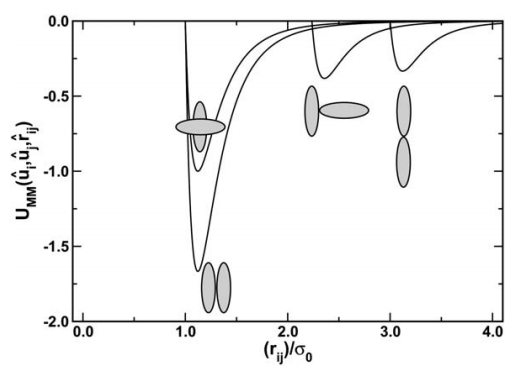
\includegraphics[width=0.7\textwidth]{gb.png}
		\caption{Behavior of the Gay-Berne potential for different 
			configurations of the two particles from \cite{moreno11} as a 
			function of the separation distance}
		\label{fig:gb}
	\end{figure}
The attractiveness of the Gay-Berne potential is its ability to simulate liquid 
crystal molecules as ellipsoidal particles rather having to specify the actual 
molecular structure atom-by-atom. Despite this simplification, the rich behavior
of liquid crystals is still observable in the molecular dynamics simulation.

\subsection*{Suspended sphere model potential}
A model similar to the pair potentials is used to model the interaction of the
liquid crystal molecules with a sphere. From \cite{lubensky98}, it reads
	\begin{equation} \label{sphere-pot}
		U_{sphere} (\hat{e}, \hat{r}) 
		= 4\epsilon_0 \left(\frac{1}{R(\hat{e}, \hat{r})}\right)^{18}
		- W\frac{
			(\hat{r}\cdot\hat{e})^6
			}
			{
			r^6
			}
	\end{equation}
where 
	\begin{equation}
		R(\hat{e}, \hat{r}) = 
		\frac{
			\sigma_s
		}
		{
			r - \sigma_r(\hat{e}, \hat{r}) + \sigma_s
		}
	\end{equation}
Here $r$ is the distance from the center of the sphere to the center of the
molecule.The positive term represents the hard repulsive force due to the
molecules colliding with the sphere itself. To model the surface anchoring there
is a similar term which gives a well like in the pair-potential. This attractive
term has been modified with a dot product between the separation vector between
the center of the sphere and the orientation of the molecules themselves. When
the vectors are completely aligned (when a liquid crystal molecule is
perpendicular to the surface of the sphere), the attractive force is at a
maximum. When the molecules are tangential to the surface, there is no 
attractive force.

The shape function describing the interaction of various configurations of the
sphere with ellipsoidal molecules is
	\begin{equation}
		\sigma_r(\hat{e}, \hat{r}) =
		\sigma_0^r\left[1-\chi_r(\hat{e} \cdot \hat{u})\right]^{-1/2}
	\end{equation}
$\chi_r$ is
	\begin{equation}
		\chi_r = 
		\frac{
			\sigma_e^2 - \sigma_s^2
		}
		{
			\sigma_e^2 + 4R_{sphere}^2
		}
	\end{equation}
$\sigma_0^r$ is given by
	\begin{equation}
		\sigma_0^r 
		= \frac{1}{\sqrt{2}}\left( \sigma_s^2 + 4R_{sphere}^2 \right)^2
	\end{equation}
	$R_{sphere}$ is the radius of the sphere. 

\subsection*{Velocity Verlet Method}
Once the forces and torques on each particle due to it's neighbors have been
calculated, the equations of motion can be numerically integrated. We have opted
to use the Velocity Verlet Method to do this. The Velocity Verlet method is a
second order method which is especially convenient because it allows us to
calculate the trajectories of the molecules using the positions and velocities
(versus other methods which use solely the position). To integrate the
translational motion. We start by calculating the velocity, $v_i$, of the
molecules at a half time step after the current time using its acceleration,
$a_i$, calculated at the current time step . 
	\begin{equation} \label{vv-v1}
		v_i(t+\frac{\Delta t}{2}) 
		= v_i(t) + a_i(t)\frac{\Delta t}{2}
	\end{equation}
The position, $x_i$, at the next time step is calculated.
	\begin{equation} \label{vv-x}
		x_i(t+\Delta t) 
		= x_i(t) + v_i(t+\frac{\Delta t}{2})\Delta t
	\end{equation}
Finally, the velocity of the next time step is calculated.
	\begin{equation} \label{vv-v2}
		v_i(t+\Delta t) 
		= v_i(t + \frac{\Delta t}{2}) 
		+ a_i(t + \frac{\Delta t}{2})\frac{\Delta t}{2}
	\end{equation}
This can be visualized diagrammatically as shown in Figure \ref{fig:vv}.
	\begin{figure}[H]
		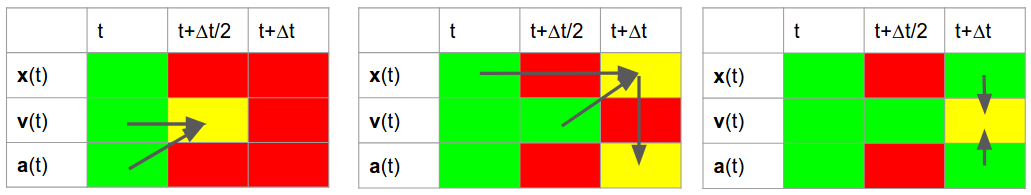
\includegraphics[width=\textwidth]{vv.png}
		\caption{A diagramatic representation of the numerical integration of
			the spatial coordinates}
		\label{fig:vv}
	\end{figure}

The orientations and angular velocities are calculated similarly, but with a
modification to constrain the orientations of the molecules to unit length and
to ensure that they are perpendicular to the angular velocities. The Velocity 
Verlet method itself does not restrict calculated quantities (position, 
velocity, orientation, angular velocity) to unit length, and Lagrange 
multipliers must be used to incorporate the conditions that the orientations
must be of unit length and perpendicular to the angular velocities into the 
equations of motion \cite{allen87}. The constraint on the length can be written 
as follows:
	\begin{equation} \label{unit-length}
		e_i(t+\Delta t)  \cdot e_i(t+\Delta t) = 1
	\end{equation}
where for calculating the Lagrange multiplier we let
	\begin{equation} \label{vv-e}
		e_i(t+\Delta t) 
		= e_i(t) 
		+ u_i(t + \frac{\Delta t}{2})\Delta t 
		+ \lambda e_i(t) \Delta t
	\end{equation}
$u_i$ is the angular velocity of the molecule. The resulting Lagrange multiplier 
is 
	\begin{equation} \label{lagrange-1}
		\begin{align}
			\lambda 
			& = -\left(\hat{e}(t) 
				\cdot \vec{u}(t+\frac{1}{2}\Delta t)+\frac{1}{\Delta t} 
			\right)\\
			& \pm \left[ 
				\left( \hat{e}(t) \cdot \vec{u}(t+\frac{1}{2}\Delta t)
				+ \frac{1}{\Delta t}
				\right)^2 
				- \vec{u}(t+\frac{1}{2}\Delta t) 
				\cdot \vec{u}(t+\frac{1}{2}\Delta t)
				- \frac{2 \hat{e}(t) \cdot \vec{u}(t+\frac{1}{2}\Delta t)}
				{\Delta t}
			\right]
		\end{align}
	\end{equation}
The constraint such that the orientations and angular velocities must be
perpendicular is calculated after the new orientations are calculated. It is
	\begin{equation} \label{eu-perp}
		e_i(t+\Delta t)  \cdot u_i(t+\Delta t)  = 0
	\end{equation}
where 
	\begin{equation} \label{vv-u}
		u_i(t+\Delta t) = u_i(t+\frac{\Delta t}{2}) 
		+ \alpha_i(t+\Delta t)\frac{\Delta t}{2} 
		+ \tilde{\lambda} e_i(t+\Delta t)\frac{\Delta t}{2}
	\end{equation}
$\alpha_i$ is the angular acceleration of the molecule. The second Lagrange
multiplier is
	\begin{equation} \label{lagrange-2}
		\begin{align}
			\tilde{\lambda} 
			= \frac{2}{\Delta t} \vec{u}(t + \frac{1}{2}\Delta t) 
			\cdot \hat{e}(t+\Delta t) 
			+ \vec{\alpha}(t + \Delta t) \cdot \hat{e} (t + \Delta t)
		\end{align}
	\end{equation}
After finding the Lagrange multipliers, integrating the equations of motion for
the rotational motion is analogous to the translational motion.

Additionally in order to keep the temperature constant in the simulation, a
thermostat from \cite{ilnytskyi02} is used to adjust the velocities. This keeps 
the fluctuations of the local average orientations to a minimum.

\subsection*{Initialization}
When the simulation is initialized, it is important to make sure the that 
particles are not too densely packed. This can result in a large repulsive force
causing particles to scatter off at high velocity producing errors in position 
or energy calculations. A simple way of avoiding this situation, is to 
initialize the positions of each particle such that they are arranged in a 
periodic structure within the simulation box. The side lengths of the simulation
box and the number of particles is dependent on the desired density of
particles. After each particle is placed on a lattice site, the next step is to
assign random velocities from a uniform distribution for each degree of freedom.
At this point, the sum of the velocities and the sum of the squares of the
velocities are calculated. Two adjustments need to be made before the
initialization process is complete. First, the velocity of the system's center
of mass is set to zero. The center of mass velocity is calculated by dividing
the total velocities for each component by the number of particles. For each
particle, the velocities in each direction are shifted by subtracting the center
of mass velocity. This process prevents the system as a whole from shifting
around. The second adjustment is to set the kinetic energy of the system. The
average kinetic energy of a system can be related to the temperature by the 
following equation:
	\begin{equation}
		\langle \frac{1}{2}mv_i^2 \rangle=k_bT
	\end{equation}
From the above, a scaling factor is calculated using the sum of squared 
velocities for each degree of freedom.
	\begin{equation}
		f_{i,scaling}=\frac{k_bT}{\langle v_i^2 \rangle}
	\end{equation}
The velocity components for each particle are multiplied by the respective 
scaling factors \cite{frenkel01}. 

\subsection*{Boundary conditions}
Periodic boundary conditions are used in the simulation. This means that there 
is an periodic arrangement of the simulation box in space. The particles in the
copies of the simulation box interact with the particles in the simulation box
itself. These boundary conditions allows for the neglect of particle
interactions with a wall. The periodic boundary conditions are implemented by
adjusting particle positions as the	leave the simulation box such that they
enter from the opposite side. As seen in Figure \ref{fig:periodic}, particle 
one leaves the bottom of the simulation box and reenters from the top.
	\begin{figure}[H]
		\centering
		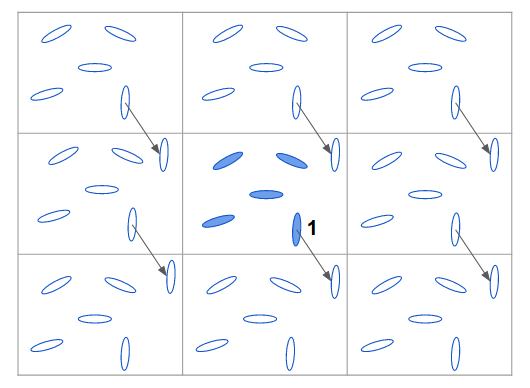
\includegraphics[width=0.7\textwidth]{periodic.png}
		\caption{Periodic boundary conditions}
		\label{fig:periodic}
	\end{figure}

\subsection*{Correlation functions}
Information about the phase and ordering of the liquid crystal as a whole can be
determined by examining correlations in positions and orientations between the
individual molecules in the system.

The pair correlation function or radial distribution function examines how the
molecules are arranged relative to each other. The function itself is
	\begin{equation}
	        g(r)=\frac{n(r)}{\rho 4 \pi r^2 dr}
	\end{equation}
where $\rho$ is the density of the system and $dr$ is the width of a spherical
shell. $n(r)$ is the number of particles in a spherical shell of radius $r$ with
some width $dr$. Essentially, the number of particles, $n(r)$, in the spherical
shell is divided by the amount of particles that would have been in the shell
had the particles been randomly distributed like in a gas. The radial
distribution function is then a comparison at each radius $r$ from a particle 
of the distribution of particles in the system to a random distribution of 
particles. 

The orientation correlation function examines how the molecules are oriented
relative to each other. It is
	\begin{equation}
		o(r) = \frac{1}{N(shell)}\sum S
	\end{equation}
where
	\begin{equation}
		S = \frac{3\cos^2(\theta)-1}{2}
	\end{equation}
In both the isotropic and nematic phase, it is expected that the particles are
mostly aligned with its nearest neighbors. The difference being that in the
nematic phase we expect to see the orientation correlation function never
decaying to zero which indicates long range ordering in the liquid crystal 
\cite{frenkel01}.
		
\section*{Simulation}
The simulation was performed with 4096 molecules with a density of 0.31 and
temperature of 0.8. The simulation was performed with
dimensionless units with $\sigma_s=1$ and $\epsilon_s=1$ and $m=1$ ($m$ is the
mass of the particles. The rest of the quantities are scaled based of these
three quantities \cite{frenkel01}.

For the first 25000 timesteps, system is equillibriated and allowed to form a
nematic phase without the sphere model potential turned on. After this point, a
space is carved out for the sphere by removing particles in a sphere with
$R_{sphere}=3$. The sphere model terms are then turned on with a cutoff distance
of $3\sigma_s$. Interestingly enough, and expected, despite the sphere model
acting only on particles in its direct vicinity, there are long range
distortions of the director field. The system is allowed to equillibriate for
75000 timesteps. Towards the end of the simulation the average of the Q-tensor
is calculated which is used later to plot the director field and look at the
biaxiality. Additionally, the pair and orientation correlation functions are
calculated.

\section*{Results}

\subsection*{Verification of liquid crystalline behavior}
Before adding the sphere to the simulation, it must be confirmed that there is
actually a liquid crystal phase and, particularly, the nematic phase. That means
that three properties must be observed. The first is that ordering increases as
the temperature in the simulation decreases. Figure \ref{fig:phase} is a plot of
the scalar order parameter for the liquid crystal at various temperatures.
	\begin{figure}[H]
		\centering
		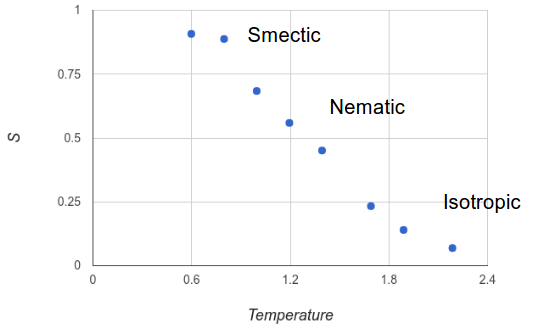
\includegraphics[width=0.8\textwidth]{phase.png}
		\caption{The scalar order parameter for a range of temperatures}
		\label{fig:phase}
	\end{figure}
As seen, three distinct phases where found to exist using the Gay-Berne 
potential to model the ellipsoidal liquid crystal molecules. The nematic phase
characterized by $S$ being between 0.3 and 0.7 was found at temperatures between
0.8 to 1.3.

Another feature we would like to see is peaks in the pair correlation function.
In an isotropic fluids, molecules like to organize into spherical shells about
each other. In the pair correlation function, this manifests as periodically
spaced peaks. The same liquid structure should be observed in the liquid
crystal. Figure \ref{fig:pcf} is a plot of the pair correlation function
for the simulation at temperature 0.8.
	\begin{figure}[H]
		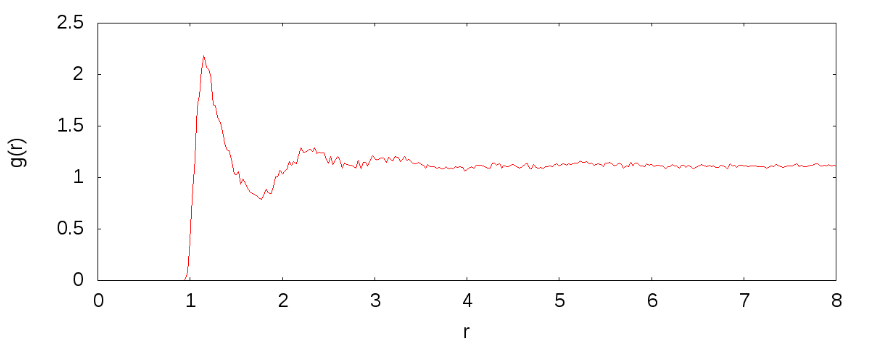
\includegraphics[width=\textwidth]{pcf.png}
		\caption{The pair correlation function for the nematic liquid crystal
		without a sphere inserted}
		\label{fig:pcf}
	\end{figure}
At least two peaks are able to be resolved in the simulation which indicated
that a liquid is being simulated.

Long range orientational ordering must also be observed. This confirms that a
nematic phase is being simulated. Figure \ref{fig:ocf} is the orientation
correlation function for temperature 0.8.
	\begin{figure}[H]
		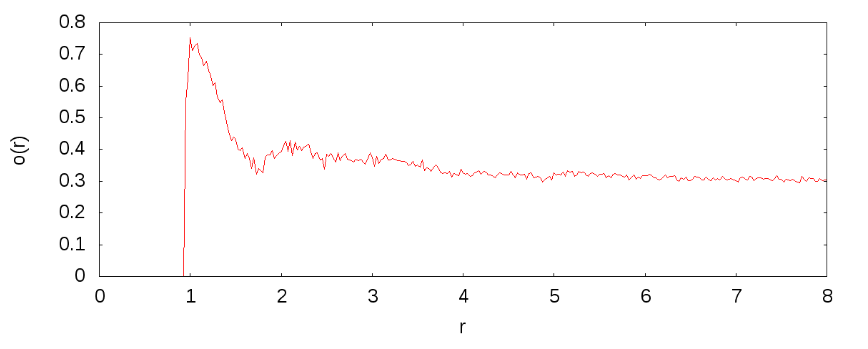
\includegraphics[width=\textwidth]{ocf.png}
		\caption{The orientation correlation function for the nematic liquid
		crystals without a sphere inserted}
		\label{fig:ocf}
	\end{figure}
As seen, the scalar order parameter is quite high for the nearest neighbors of
particles. The function decays but remains about 0.35 for long distances which
means that there is indeed long range ordering between the molecules.

\subsection*{Director field plots and defects}
In order to visualize the orientations of the molecules and find defects, the 
director field is plotted. The simulation box is divided into a 11 by 11 by 11
grid. In each bin, the Q-tensor is averaged for 50 timesteps. After the
simulation is complete, the tensors are diagonalized giving the local average
orientation and the biaxiality in the bin. Figure \ref{fig:biaxial-3d} is a 3D
plot of the local preferred orientation of the molecules colored according to
the amount of biaxiality in the bin.
	\begin{figure}[H]
		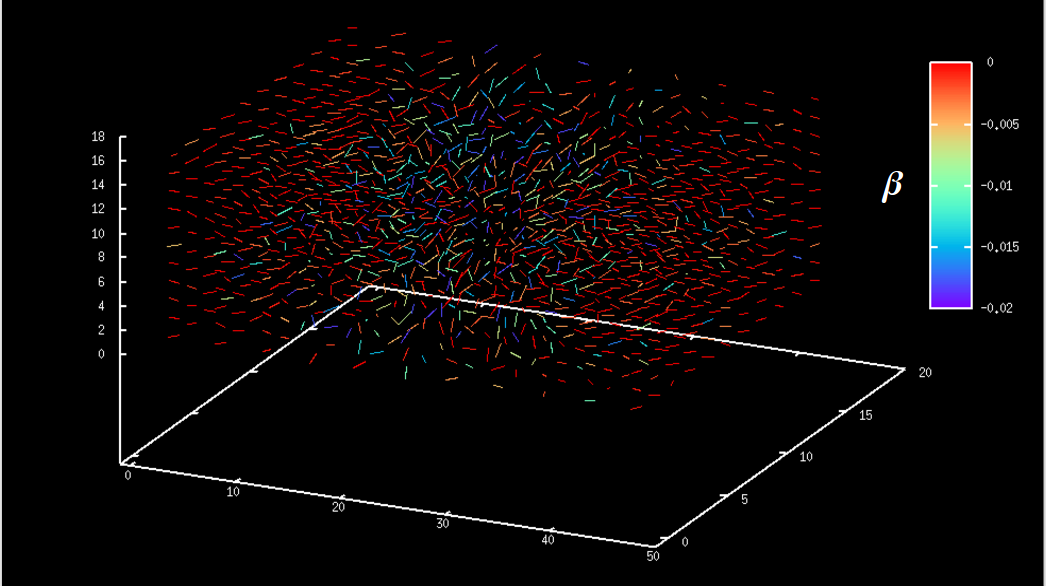
\includegraphics[width=\textwidth]{biaxial-3d.png}
		\caption{A 3-D plot of the director field with the sphere inserted}
		\label{fig:biaxial-3d}
	\end{figure}
The closer to the sphere the more biaxial the liquid crystal becomes. Far away
the molecules are mostly uniaxial which is a good indicator that the director is
deforming to match back up with the boundary conditions. This indicates
locations in the liquid crystal where there may be more than one preferred axis 
of orientation and defects.

To get a better idea of the behavior of the liquid crystal at the surface of the
sphere a 2D slice along the short face of the simulation box is taken in figure
\ref{fig:biaxial-2d}.
	\begin{figure}[H]
		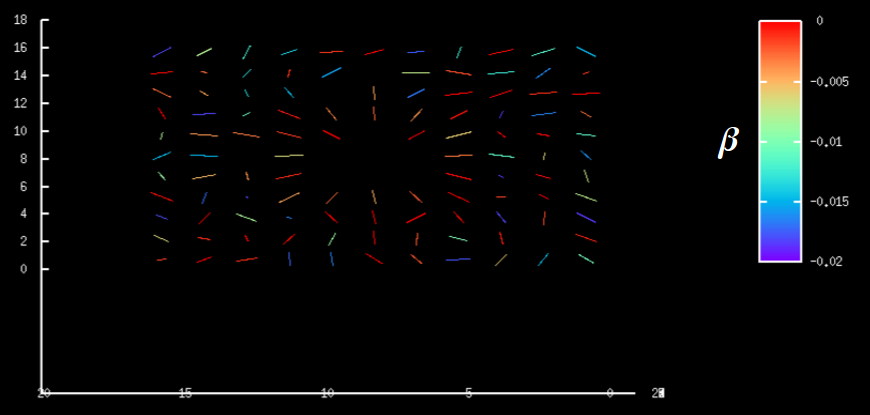
\includegraphics[width=\textwidth]{biaxial-2d.png}
		\caption{A slice of the director field with the sphere inserted}
		\label{fig:biaxial-2d}
	\end{figure}
Radial anchoring at the surface of the sphere is apparent. This means the sphere
model potential is working correctly.

\subsection*{Measurement of defect radius}
In Figure \ref{fig:biaxial-2d} there is a ring of biaxiality that extends to the
edges of the simulation box which may be an indication of a line defect forming
around the sphere. Unfortunately, the director field does not deform back into a
uniaxial phase at the boundaries. Despite using periodic boundary conditions,
the hope was that the images would push on each other and constrain the
orientations of the molecules at the sides of the simulation box. The fact that
the biaxiality extends to the end of the simulation box makes it hard to
estimate the size of the defect ring.

Additionally, a line defect around the sphere is being observed instead of a
point defect as seen in experiment. This is likely do to the fact that the
sphere in the simulation is not large enough \cite{lubensky98}

\section*{Conclusion}
Using the Gay-Berne potential, a liquid crystal in the nematic phase has been
simulated. Several liquid crystal phases have been observed along with liquid
like structure. By adding a potential to model and immersed sphere, radial
anchoring of the molecules on the sphere has been observed. There is some
indication that a line defect has formed around the sphere, but due to the
constraints of the simulation box size it is not possible to make an estimation
of the distance between the surface of the sphere and the defect. Further
studies will require a larger simulation box and, thus, more particles and more
simulation time. 

\section*{Acknowledgements}
Foremost, I would like to thank Professor Jorge Vi\~nals for the guidance he has
provided while constructing the simulation and during way too many hours of
debugging. Thank you to Professor Paul Crowell for organizing the physics honors
seminar where we were able to showcase our work during presentations. Finally,
the University of Minnesota Honors Department deserves recognition for giving 
undergraduates the opportunity to perform research for and write theses such as 
this one.

%------------------------------------------------------------------------------%
%--------------------------------  References  --------------------------------%
%------------------------------------------------------------------------------%

\bibliography{mybib, revtek-custom}{}
\bibliographystyle{apsrev4-1}

\end{document}
%------------------------------------------------------------------------------&
